\documentclass[12pt,a4paper]{article}

% --------------------------------------------------
% JEZIK IN KODIRANJE
% --------------------------------------------------
\usepackage[utf8]{inputenc}
\usepackage[T1]{fontenc}
\usepackage[slovene]{babel}

% --------------------------------------------------
% POSTAVITEV STRANI
% --------------------------------------------------
\usepackage[a4paper,margin=2.5cm]{geometry}
\usepackage{setspace}
\onehalfspacing

% --------------------------------------------------
% MATEMATIKA
% --------------------------------------------------
\usepackage{amsmath}
\usepackage{amssymb}

% --------------------------------------------------
% TABELE, SLIKE IN GRAFI
% --------------------------------------------------
\usepackage{array}
\newcolumntype{L}[1]{>{\raggedright\arraybackslash}p{#1}}
\newcolumntype{R}[1]{>{\raggedleft\arraybackslash}p{#1}}
\usepackage{booktabs}
\usepackage{graphicx}
\graphicspath{{slike/}}
\usepackage{pgfplots}
\pgfplotsset{compat=1.18}
\usepackage{enumitem}
\setlist[itemize]{itemsep=0.2em,topsep=0.3em}

% --------------------------------------------------
% POVEZAVE
% --------------------------------------------------
\usepackage{xurl}
\usepackage[hidelinks]{hyperref}

% --------------------------------------------------
% CITIRANJE
% --------------------------------------------------
\usepackage[round,authoryear]{natbib}
\addto\captionsslovene{\renewcommand{\refname}{Viri}}

% --------------------------------------------------
% ODSTAVKI
% --------------------------------------------------
\setlength{\parindent}{0pt}
\setlength{\parskip}{0.7em}

% --------------------------------------------------
% NASLOV
% --------------------------------------------------
\title{\textbf{Investicije v razvoj umetne inteligence: ali so pričakovanja donosov upravičena?}}
\author{}
\date{}

\begin{document}

\maketitle

% ==================================================
\section{Uvod}
% ==================================================

% --------------------------------------------------
\subsection{Širša problematika}
% --------------------------------------------------

Ali nova tehnologija prinese rast produktivnosti, je staro vprašanje makroekonomije. Robert Solow je leta 1987 zapisal, da računalniško dobo vidimo povsod, razen v statistiki produktivnosti; temu pravimo Solowov paradoks. Rast produktivnosti dela v ZDA se je ob hitri računalniški opremljenosti upočasnila s 3~\% v šestdesetih na okoli 1~\% v osemdesetih, nato pa se je med letoma 1995 in 2005 spet pospešila. Brynjolfsson, Rock in Syverson zamik pojasnjujejo s »produktivnostno J-krivuljo«: nova tehnologija zahteva veliko dopolnilnih, večinoma neopredmetenih vlaganj (nova organizacija dela, usposabljanje, programska oprema), ki jih statistika sprva ne zajame. Izmerjena produktivnost zato najprej stagnira ali celo upade, šele pozneje pa močno naraste. Isto vprašanje se danes postavlja za umetno inteligenco (UI) \citep{ChicagoBoothReview}.

\begin{figure}[htbp]
\centering
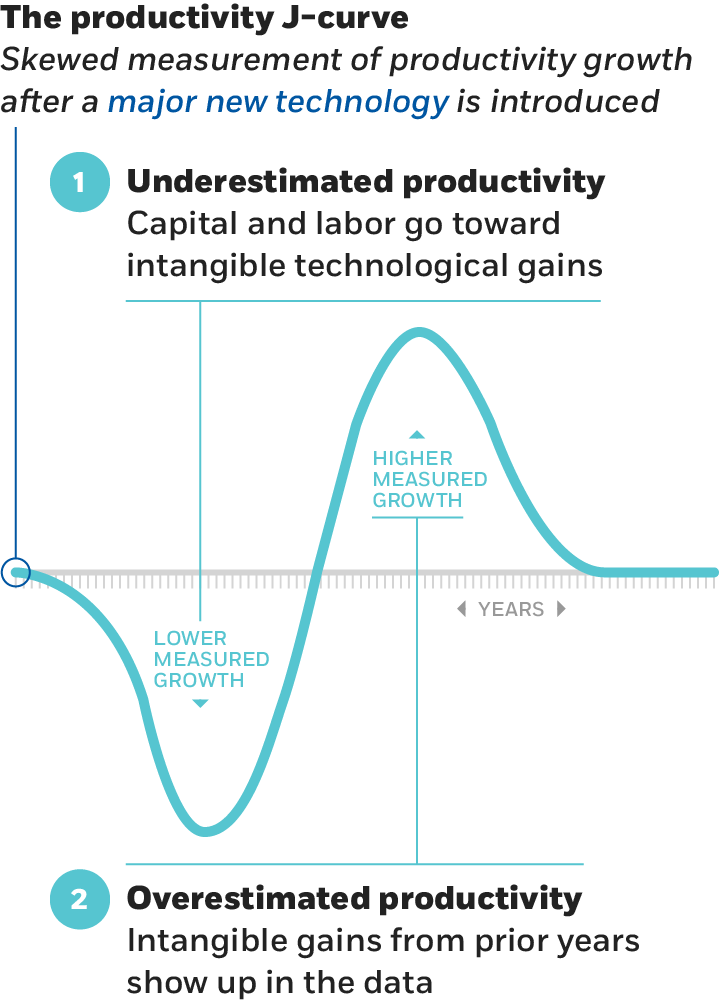
\includegraphics[width=0.4\textwidth]{image1.png}
\caption{Produktivnostna J-krivulja. Vir: \citep{ChicagoBoothReview} (po Brynjolfsson, Rock, Syverson, 2021)}
\label{fig:jkrivulja}
\end{figure}

Velika ameriška tehnološka podjetja (Amazon, Microsoft, Alphabet in Meta) za leto 2026 načrtujejo okoli 730 milijard dolarjev kapitalskih izdatkov, kar je približno 78~\% več kot okoli 410--416 milijard dolarjev leta 2025. Po ocenah so leta 2023 porabila okoli 155 milijard, leta 2024 pa okoli 251 milijard dolarjev. Viri se v zaokrožitvah malo razlikujejo (Forbes navaja 700--725 milijard dolarjev, druge zbirke do 750), predvsem zaradi obravnave finančnih najemov in Microsoftovega fiskalnega leta \citep{ValueAddVC,Forbes2026,Platformonomics2025,Platformonomics2026}.

\begin{figure}[htbp]
\centering
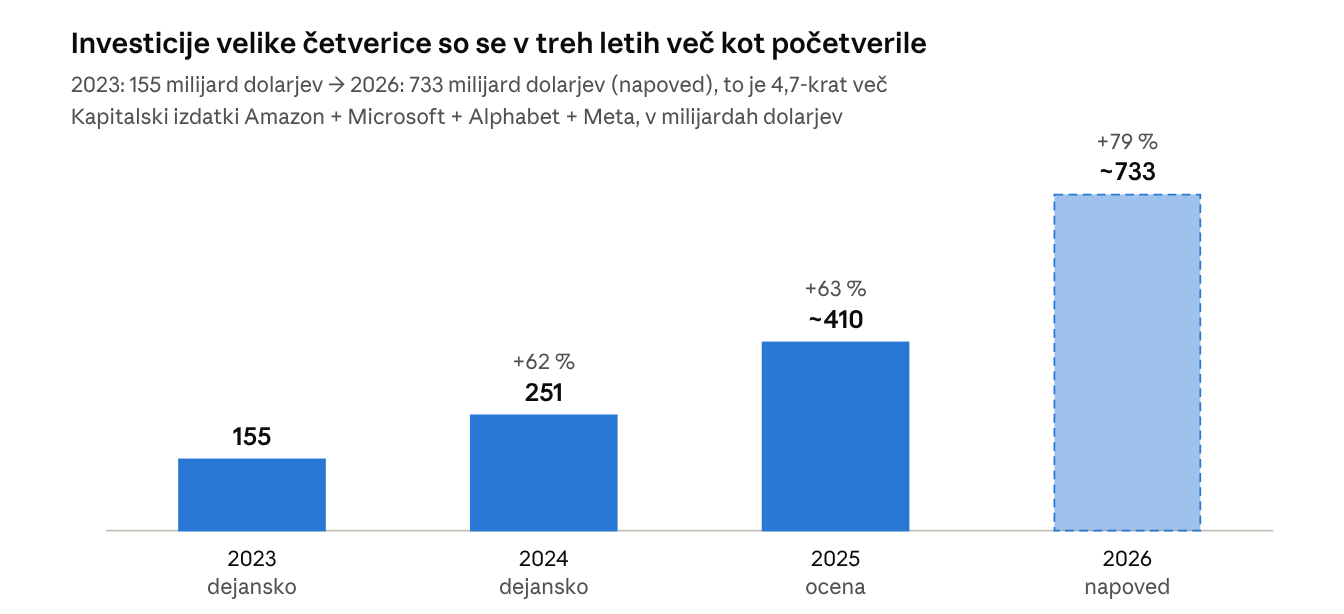
\includegraphics[width=\textwidth]{image2.png}
\caption{Platformonomics (2023--2024), medijske ocene (2025), poročila podjetij in zbirke napovedi (2026) · glej Viri}
\label{fig:capex}
\end{figure}

Ta obseg je makroekonomsko pomemben, ker so investicije nihajoča komponenta BDP in določajo dinamiko kapitala. Po oceni ING je široko opredeljena tehnološka investicija (oprema za obdelavo informacij, programska oprema in podatkovni centri) v drugem četrtletju 2026 pojasnjevala okoli polovico medletne rasti ameriškega BDP, pri ožji opredelitvi okoli tretjino. Flossbach von Storch opozarja, da je rezultat zelo odvisen od opredelitve: investicije v UI so glede na definicijo 2,3--8,2~\% BDP. Ameriški urad za ekonomsko analizo (BEA) postavke »UI« ne objavlja, zato so vsi ti deleži ocene \citep{ING,FlossbachVonStorch}. Najnovejši podatki o produktivnosti so mešani: v ameriškem nekmetijskem poslovnem sektorju je v drugem četrtletju 2026 zrasla za 1,4~\% (letna stopnja), medletno pa za 2,2~\%. Ali je to že učinek UI, ostaja odprto \citep{BLSProductivity2026}.

% --------------------------------------------------
\subsection{Pomen: zakaj je vprašanje o donosih pomembno}
% --------------------------------------------------

\textbf{Možen balon.} Naložbe se vse bolj financirajo z zunanjim kapitalom. Po analizi dveh ekonomistov s Stanforda je vrzel med porabo in prihodki od UI od leta 2024 skoraj 1000 milijard dolarjev. Nasproti tej skrbi stoji močno povpraševanje: prihodki Amazonovega AWS so v drugem četrtletju 2026 zrasli za 37~\% na 42,2 milijarde, Google Cloud pa za 82~\% na 24,8 milijarde dolarjev \citep{Alphabet2026,Amazon2026,Meta2026,Axios2026}.

\begin{figure}[htbp]
\centering
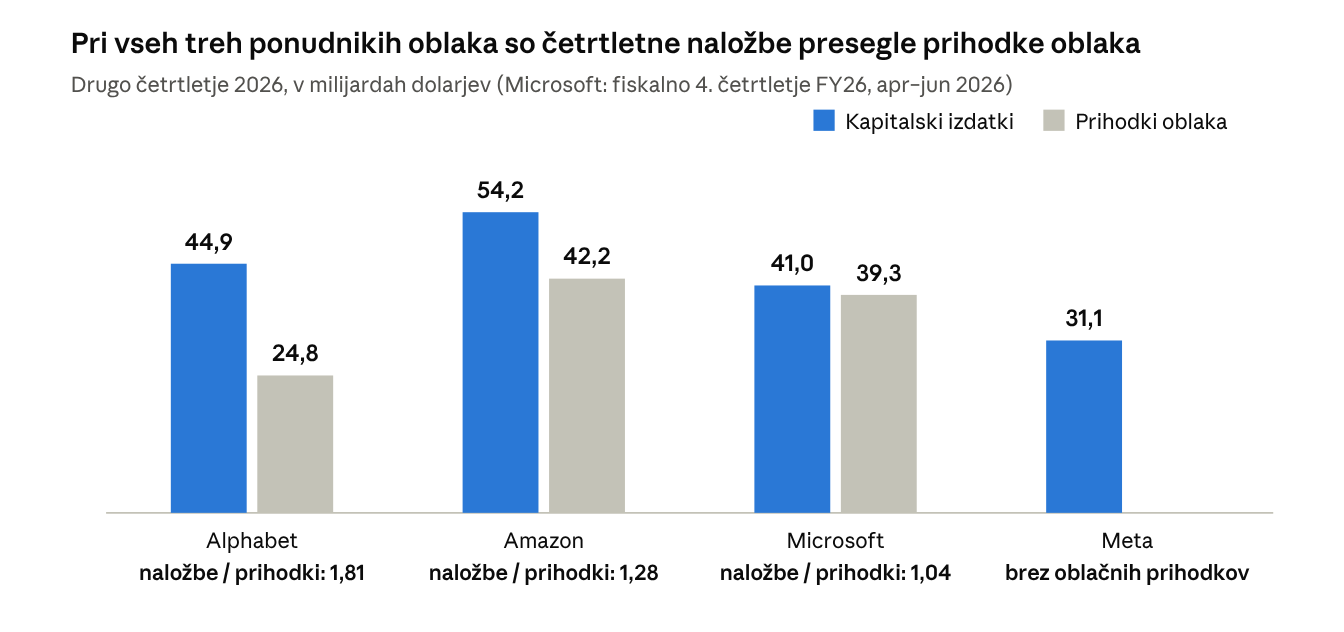
\includegraphics[width=0.9\textwidth]{image3.png}
\caption{Sporočila za javnost Alphabet (22. 7. 2026), Amazon (30. 7. 2026), Meta (29. 7. 2026); Microsoft po medijskih poročilih o rezultatih FY26 Q4}
\label{fig:oblak}
\end{figure}

Graf je le grob namig: prihodki oblaka niso prihodki od UI, kapitalski izdatki pa niso samo UI. Pomembna protiutež so naročila: Google Cloud poroča o stanju naročil okoli 514 milijard dolarjev, Microsoft pa o komercialnih preostalih pogodbenih obveznostih 678 milijard. To so pogodbene zaveze, ne dobiček; ali bodo prinesle donos nad $r + \delta$, je jedro naloge. Microsoftove številke izhajajo iz prepisa klica z vlagatelji \citep{TheNextWeb2026,Redmond2026,MicrosoftFY26Q4Call}.

\textbf{Alokacija kapitala.} Če so naložbe v UI predimenzionirane, se redki viri (kapital, čipi, električna energija, strokovnjaki) preusmerjajo iz uporab z višjim donosom. Del rasti izdatkov ne pomeni več zmogljivosti, ampak višje cene: Microsoft naj bi okoli 25 milijard dolarjev svojega proračuna za 2026 pripisal dražjim komponentam. Mejni produkt vsakega dodatnega dolarja je zato lahko nižji, kot kažejo skupni zneski \citep{Forbes2026}.

\textbf{Vpliv na rast.} Ker UI investicije bistveno prispevajo k rasti BDP, bi njihovo umikanje rast neposredno znižalo: Flossbach von Storch ocenjuje začetno izgubo na okoli 0,7 odstotne točke rasti realnega BDP. Dolgoročno pa rast ne poganja obseg naložb, ampak produktivnost, ki jo te naložbe omogočijo \citep{FlossbachVonStorch}.

% --------------------------------------------------
\subsection{Konkretni primer: ZDA, 2022--2026}
% --------------------------------------------------

Naloga obravnava štiri ameriške ponudnike oblaka in UI: Amazon, Microsoft, Alphabet in Meta. Izbrana so, ker so med največjimi vlagatelji v UI (skupaj načrtujejo okoli 730 milijard dolarjev kapitalskih izdatkov v letu 2026) in ker so javno kotirana, zato objavljajo preverljive podatke (obrazca 10-Q in 10-K pri ameriškem regulatorju SEC). Poslovni modeli se razlikujejo: Amazon, Microsoft in Alphabet zmogljivost prodajajo prek oblaka (AWS, Azure, Google Cloud), Meta pa jo uporablja predvsem za oglaševanje. Spodnji graf kaže, da se izdatki za UI med podjetji precej razlikujejo \citep{SECEdgar,ValueAddVC}.

\begin{figure}[htbp]
\centering
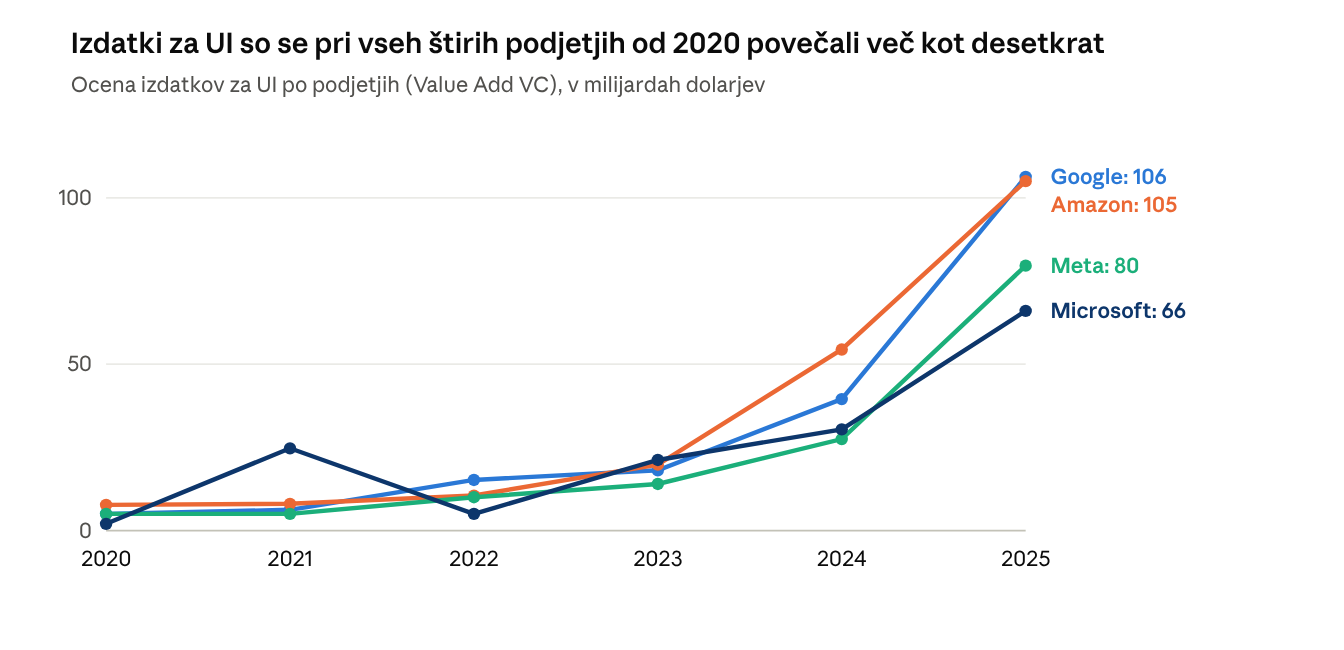
\includegraphics[width=\textwidth]{image4.png}
\caption{Value Add VC: ocena izdatkov za UI po podjetjih (infrastrukturni capex, povezan z UI, prevzemi, kapitalski deleži in pogodbe) · ni enako skupnemu capexu}
\label{fig:izdatki}
\end{figure}

Podatki so ocena izdatkov za UI (infrastrukturni capex, povezan z UI, prevzemi, kapitalski deleži in pogodbe), zato niso enaki skupnemu capexu s prejšnjega grafa. Skok Microsofta leta 2021 odraža prevzem podjetja Nuance (19,7 milijarde dolarjev) \citep{ValueAddVC}.

Za zanimivost omenimo Kitajsko: tam je slika drugačna, saj se izdatki za UI poročajo in štejejo drugače kot v ZDA, podatki pa so manj primerljivi. ByteDance je na primer zasebno podjetje, zato se ocene njegovih letošnjih izdatkov gibljejo od okoli 29 do 59--74 milijard dolarjev. Zaradi tega Kitajske v analizo ne vključujemo \citep{BigGo,AsiaTechReview}.

Obdobje 2022--2026 je izbrano, ker 2022 pomeni izhodišče pred širitvijo generativne UI, 2026 pa je prvo leto, za katero so na voljo napovedi podjetij in rezultati prvega polletja. Podatki veljajo do sredine oktobra 2026; poročila za tretje četrtletje bodo objavljena konec oktobra.

% --------------------------------------------------
\subsection{Opredelitev pojmov}
% --------------------------------------------------

\textbf{Investicije v UI} merimo s kapitalskimi izdatki (capex) štirih podjetij: z nakupi strežnikov s pospeševalniki (GPU, lastni čipi) in omrežne opreme ter z gradnjo podatkovnih centrov. V izrazoslovju predavanj gre za bruto investicije $I_t$. Capex ni samo UI (npr. Amazonova logistika), zato podatke razumemo kot zgornjo mejo naložb v UI.

\textbf{Donos} pri podjetjih merimo s prihodki in dobičkom oblačnih segmentov (AWS, Azure, Google Cloud) ter s pogodbenimi naročili. Prihodek pa še ni donos na kapital: v modelu mora mejni produkt kapitala $F'(K)$ presegati $r + \delta$. Pri gospodarstvu je donos rast produktivnosti dela (BLS), ki se v statistiki pokaže z zamikom (J-krivulja) \citep{BLSLabourProductivity}.

\textbf{Življenjska doba opreme ($\delta$)} je pri UI kratka: po besedah Microsoftove finančne direktorice Amy Hood je bilo okoli dve tretjini kapitalskih izdatkov v zadnjem četrtletju šlo za kratkožive naložbe, predvsem procesorje in grafične pospeševalnike, kar dviguje prag donosnosti \citep{MicrosoftFY26Q4Call}.

% --------------------------------------------------
\subsection{Struktura naloge}
% --------------------------------------------------

Iz tega izhaja vprašanje, ki ga obravnava naloga: ali pričakovani donosi investicij v razvoj umetne inteligence upravičujejo sedanji obseg naložb? Osredotočile se bomo na ZDA in omenjena štiri podjetja, vprašanje pa bomo navezale na dva modela: model uporabniških stroškov kapitala (mejni produkt kapitala mora presegati $r + \delta$, z neto sedanjo vrednostjo) in njegovo razširitev s Tobinovim q.


% ==================================================
\section{Tobinov q kot razmerje med tržno vrednostjo in nadomestitveno vrednostjo}
% ==================================================

% ==================================================

\subsection{Opredelitev Tobinovega q}

% ==================================================

Tobinov q je ekonomski kazalnik, ki povezuje \textbf{tržno vrednost podjetja oziroma njegovega kapitala z nadomestitvenimi stroški tega kapitala}. Njegov osnovni namen je pokazati, kako je vrednost kapitala, kot jo ocenjuje trg, primerljiva s stroškom, ki bi bil potreben za ponovno vzpostavitev oziroma nadomestitev tega kapitala. V najpreprostejši obliki ga lahko zapišemo kot:

\begin{equation}
q = \frac{\text{tržna vrednost kapitala}}{\text{nadomestitvena vrednost kapitala}}.
\end{equation}

Pri tem je pomembno razlikovati med \textbf{povprečnim q} in \textbf{mejnim oziroma marginalnim q}. Povprečni q primerja celotno tržno vrednost podjetja oziroma njegovega kapitala s celotno nadomestitveno vrednostjo kapitala. Mejni q pa primerja vrednost \emph{dodatne enote kapitala} z njenim nadomestitvenim stroškom. Prav mejni q je v teoretičnem modelu pomemben za odločanje o novih investicijah. Hayashijeva formalizacija pokaže, da je pod določenimi predpostavkami mogoče marginalni q povezati s povprečnim q, ki ga je v praksi precej lažje opazovati \citep{AndreiMannMoyen2017,PetersTaylor2016}.

Logika kazalnika je relativno preprosta. Če je $q>1$, je tržna vrednost kapitala višja od stroška njegove nadomestitve. To pomeni, da trg podjetju oziroma njegovemu kapitalu pripisuje višjo vrednost, kot bi znašal strošek ustvarjanja primerljivega kapitala. V osnovnem investicijskem modelu to ustvarja spodbudo za dodatne investicije. Če je $q<1$, je situacija obrnjena: tržna vrednost kapitala je nižja od njegove nadomestitvene vrednosti, zato je ekonomska spodbuda za ustvarjanje dodatnega kapitala šibkejša. Pri $q \approx 1$ je tržna vrednost kapitala približno enaka strošku njegove nadomestitve.

Zato lahko Tobinov q razumemo kot \textbf{formalno povezavo med vrednotenjem kapitala in investicijsko odločitvijo}. Ne pove neposredno, ali bo neka investicija uspešna, ampak omogoča primerjavo med vrednostjo, ki jo kapital ustvarja oziroma ji jo pripisuje trg, in stroškom njegovega ustvarjanja.

Pri tem je pomembno, da Tobinov q ni enak klasičnemu računovodskemu kazalniku donosnosti. Ne meri neposredno dobička na vloženi evro in tudi ne predstavlja klasičnega kazalnika ROI. Njegova posebnost je v tem, da na eni strani uporablja \textbf{tržno vrednost}, na drugi pa \textbf{nadomestitveno vrednost kapitala}. V literaturi se Tobinov q zato uporablja kot merilo investicijskih priložnosti podjetja \citep{PetersTaylor2016}.

\begin{table}[htbp]

\centering

\caption{Osnovna interpretacija Tobinovega q}

\label{tab:interpretacija_q}

\begin{tabular}{p{3cm}p{10cm}}

\toprule

\textbf{Vrednost q} & \textbf{Interpretacija} \\\\

\midrule

$q>1$ &

Tržna vrednost kapitala je višja od nadomestitvenega stroška, zato obstaja večja ekonomska spodbuda za nove investicije. \\\\

$q\approx1$ &

Tržna vrednost kapitala je približno enaka nadomestitvenemu strošku. \\\\

$q<1$ &

Tržna vrednost kapitala je nižja od nadomestitvenega stroška, zato je spodbuda za nove investicije šibkejša. \\\\

\bottomrule

\end{tabular}

\end{table}

% ==================================================

\subsection{Povezava Tobinovega q z investicijami}

% ==================================================

Povezava med $q$ in investicijami izhaja iz vprašanja, ali se podjetju splača povečati svoj kapital (kapital je vse, kar podjetje uporablja za proizvodnjo dobrin ali storitev in kar mu omogoča ustvarjanje prihodnjih prihodkov). Če pričakovana vrednost, ki jo podjetju prinese dodatna enota kapitala, presega strošek njene pridobitve, je investicija za podjetje ekonomsko smiselna.

To lahko ponazorimo na primeru podjetja \textbf{Amazon}. Amazon je imel konec leta 2025 približno \textbf{818 milijard dolarjev sredstev}, medtem ko je bila njegova tržna vrednost približno \textbf{2,47 bilijona dolarjev}.

Če za poenostavljen približek uporabimo razmerje med tržno vrednostjo podjetja in vrednostjo njegovih sredstev, dobimo:

\begin{equation}
q = \frac{2.470}{818} \approx 3,02.
\end{equation}

Torej je $q$ večji od 1. To pomeni, da je bila tržna vrednost Amazona približno trikrat višja od vrednosti njegovih bilančnih sredstev. Visoka vrednost $q$ lahko kaže, da trg podjetju pripisuje pomembno prihodnjo vrednost, ki ni v celoti zajeta v njegovi obstoječi fizični in računovodsko izkazani osnovi kapitala.

Za primerjavo lahko pogledamo \textbf{Delta Air Lines}. Konec leta 2025 je imela Delta približno \textbf{81,3 milijarde dolarjev sredstev}, njena tržna vrednost pa je znašala približno \textbf{45,3 milijarde dolarjev}.

V tem primeru dobimo:

\begin{equation}
q = \frac{45,3}{81,3} \approx 0,56.
\end{equation}

Torej je $q$ manjši od 1. V tem primeru je bila tržna vrednost podjetja nižja od vrednosti njegovih bilančnih sredstev, kar kaže na precej bolj zadržano tržno vrednotenje podjetja.

V prvem primeru je razmerje med tržno vrednostjo in vrednostjo kapitala \textbf{višje od 1}, medtem ko je v drugem primeru \textbf{nižje od 1}.
Pri Tobinovem q je zato pomembna predvsem \textbf{mejna vrednost kapitala}. Podjetje se ne odloča samo na podlagi tega,
koliko je vreden njegov obstoječi kapital, temveč predvsem na podlagi tega, kakšno vrednost bo ustvarila dodatna investicija.

%Teorija q investicij predpostavlja povezavo med tržno vrednostjo podjetij in njihovo investicijsko aktivnostjo. 

Hayashijeva formalizacija je pomembna zato, ker pokaže, pod katerimi pogoji je  marginalni q možno povezati s povprečnim q,
ki ga je  empirično lažje izračunati (marginalni q je tudi bolj relevanten če se podjetje sprašuje o tem ali naj naredi novo investicijo).
\citep{AndreiMannMoyen2017}.

To je posebej pomembno pri novih tehnologijah. Pri tehnologiji, kot je umetna inteligenca, investicije niso
omejene samo na nakup fizične opreme. Potrebni so tudi podatkovni centri, računalniška oprema, čipi, programska oprema,
podatki, raziskave in razvoj ter znanje zaposlenih. Zato je težje primerjati vrednost kapitala investiranega v AI podjetje, 
kot pa vrednost klasičnega fizičnega kapitala nekega naprimer gradbenega podjetja.

%Zato je pri AI težje določiti natančno nadomestitveno vrednost kapitala

%Tu je mišljeno predvsem primerjava med AI-kapitalom in klasičnimi fizičnimi sredstvi podjetja.

Prav tukaj se pojavi ena izmed pomembnih omejitev uporabe Tobinovega q pri umetni inteligenci.

% ==================================================

\subsection{Tobinov q in investicije v razvoj umetne inteligence}

% ==================================================

Naša osrednja tema je vprašanje \textit{»Investicije v razvoj umetne inteligence: ali so pričakovanja donosov upravičena?«}
Tobinov q nam pri tem omogoča preučevati, ali je visoka tržna vrednost podjetij, ki veliko vlagajo v AI, skladna z vrednostjo njihovega kapitala.

V zadnjih letih so investicije v umetno inteligenco hitro naraščale. Stanfordov AI Index 
za leto 2026 ugotavlja, da je globalna zasebna investicija v AI leta 2025 dosegla približno 
344,66 milijarde USD, pri čemer je bila rast posebej izrazita pri generativni umetni 
inteligenci \citep{StanfordAIIndex2026}. OECD hkrati ugotavlja, da so podjetja, povezana 
z AI infrastrukturo in gostovanjem, leta 2025 prejela približno 109,3 milijarde USD 
tveganega kapitala \citep{OECD2026}.

Tako velike investicije postavljajo vprašanje, ali bo prihodnja ekonomska vrednost 

AI dovolj velika, da bo upravičila stroške njenega ustvarjanja. \textbf{Visok Tobinov q sam po sebi še ne pomeni, da bodo investicije donosne}, temveč kaže, da trg kapitalu 
pripisuje visoko vrednost glede na njegovo nadomestitveno vrednost. Če se bodo prihodnji 
prihodki in produktivnost dovolj povečali, se lahko visoko vrednotenje upraviči, sicer pa 
lahko pride do padca tržne vrednosti.

Pomemben del teh investicij predstavljajo tudi podatkovni centri. Federal Reserve 
ugotavlja, da je bila rast poslovnih fiksnih investicij v ZDA v veliki meri povezana 
z izgradnjo infrastrukture za podporo storitvam umetne inteligence, vključno z 
investicijami v opremo in programsko opremo \citep{FederalReserve2026}.

Tobinov q je zato uporaben kot konceptualni okvir za presojo, ali večje investicije v 
AI ustvarjajo dovolj pričakovane prihodnje vrednosti glede na stroške njihovega 
ustvarjanja.

% ==================================================

\subsection{Zakaj je Tobinov q pri AI posebej zanimiv, vendar tudi omejen}

% ==================================================

Pri umetni inteligenci je nadomestitveno vrednost kapitala težje določiti kot pri fizičnih 
sredstvih, saj velik del AI kapitala predstavljajo programska oprema, podatki, algoritmi, 
raziskave in razvoj ter znanje zaposlenih. Ti elementi niso vedno v celoti prikazani v računovodskih 
podatkih, zato lahko klasični Tobinov q daje nepopolno sliko vrednosti kapitala.
Peters in Taylor (2017) ugotavljata, da vključitev neopredmetenega kapitala izboljša \citep{PetersTaylor2016} 
razumevanje povezave med Tobinovim q in investicijami, zlasti pri podjetjih, kjer ima 
neopredmeteni kapital pomembno vlogo. To je za AI posebej pomembno, saj so prav podatki, 
programska oprema in raziskave pomemben del investicij. Andrei et al. (2019) prav tako 
ugotavljajo, da je povezava med q in investicijami pomembna pri raziskovalno intenzivnih 
podjetjih, kljub njihovemu večjemu deležu neopredmetenega kapitala \citep{AndreiMannMoyen2017}.
Zato je Tobinov q pri AI najbolje uporabljati kot analitični okvir za proučevanje 
investicij in pričakovane prihodnje vrednosti, ne pa kot samostojen dokaz, da so AI 
investicije donosne.

% ==================================================

\subsection{Kaj nam Tobinov q pove o upravičenosti investicij v AI?}

% ==================================================

Tobinov q nam zato ne more dati enostavnega odgovora \textit{»da« ali »ne«} na vprašanje, 
ali so pričakovanja donosov od AI upravičena. Lahko pa nam da jasen formalni okvir za 
razmišljanje o tem vprašanju.

Prvič, če je tržna vrednost podjetij, ki intenzivno investirajo v AI, bistveno višja od 
nadomestitvene vrednosti njihovega kapitala, je q visok. To je skladno z idejo, da trg 
pričakuje visoko prihodnjo vrednost tega kapitala. Takšno vrednotenje je lahko upravičeno, 
če bodo AI investicije povzročile dovolj visoko rast prihodkov, produktivnosti in prihodnjih 
denarnih tokov.

Drugič, visoke investicije same po sebi še ne dokazujejo visoke donosnosti. Če podjetja 
gradijo velike količine podatkovnih centrov in kupujejo drago računalniško infrastrukturo, 
mora biti prihodnja uporaba te infrastrukture dovolj velika, da upraviči stroške. Federal 
Reserve ugotavlja, da je bila v ZDA rast kapitalskih izdatkov v zadnjem obdobju močno 
povezana prav z gradnjo infrastrukture za AI \citep{FederalReserve2026}.

Tretjič, pri AI je posebej pomemben problem merjenja. Če del ustvarjenega kapitala 
predstavljajo podatki, programska oprema, organizacijsko znanje in človeški kapital, 
potem klasični izračun Tobinovega q ne zajame nujno celotne ekonomske vrednosti investicije. 
Zato je pri AI q najbolje uporabljati kot \textbf{formalni merilni okvir}, ne kot popoln 
samostojen kazalnik donosnosti.

% ==================================================

\subsection{Sklep}

% ==================================================

Tobinov q je uporaben okvir za razumevanje povezave med vrednostjo kapitala in investicijami. 
Pri \(q>1\) imajo podjetja večjo spodbudo za investiranje, saj je pričakovana vrednost kapitala 
višja od stroška njegove pridobitve. Pri AI je to še posebej zanimivo, saj velik del kapitala 
predstavljajo neopredmetena sredstva, ki jih je težje meriti. Tobinov q zato ne pove neposredno, 
ali bodo AI investicije donosne, temveč omogoča presojo, ali so tržna vrednotenja in 
pričakovanja glede prihodnje vrednosti skladna z obsegom investicij.


% ==================================================
\section{Vedenjski model: neoklasični model investicij}
% ==================================================

% --------------------------------------------------
\subsection{Postavitev problema}
% --------------------------------------------------

Raziskovalno vprašanje naloge je, ali so pričakovanja donosov naložb v umetno inteligenco (UI) upravičena. Da bi lahko presodili, kaj pomeni »upravičena«, potrebujemo merilo: koliko donosa mora naložba prinesti, da se podjetju izplača. To merilo nam da vedenjski model podjetja, ki se odloča o obsegu kapitala. Uporabimo neoklasično teorijo investicij, kot je predstavljena pri predmetu (Grobovšek, Predavanje 3; Polanec, 2014, poglavje 4), in jo razširimo s ceno opreme po Jorgensonu (Jorgenson, \citeyear{Jorgenson1963}; Hall in Jorgenson, \citeyear{HallJorgenson1967}).

Obravnavamo reprezentativno podjetje, ki vlaga v UI, na primer ponudnika oblačnih storitev (Microsoft, Amazon, Alphabet, Meta), ki gradi podatkovne centre, kupuje procesorje GPU in strežnike ter prodaja storitve UI. Model temelji na standardnih predpostavkah (s predavanj):

\begin{itemize}
\item podjetje je racionalno in maksimizira vrednost premoženja (diskontirano vsoto denarnih tokov);
\item finančni trgi so popolni: podjetje se lahko zadolži po dani obrestni meri $r$;
\item proizvodna funkcija $F(K)$ je naraščajoča in konkavna (mejni produkt kapitala pada z obsegom kapitala);
\item kapital se obrablja po stopnji $\delta$, torej $K_{t+1} = (1 - \delta) \cdot K_t + I_t$.
\end{itemize}

% --------------------------------------------------
\subsection{Izpeljava modela}
% --------------------------------------------------

Podjetje v vsakem obdobju ustvari denarni tok $D_t = F(K_t) - I_t - \phi_t$, kjer so $\phi$ eksogeni fiksni stroški. Vrednost podjetja je diskontirana vsota teh tokov. Če investicije izrazimo iz dinamike kapitala, $I_t = K_{t+1} - (1 - \delta)K_t$, in vrednost odvajamo po kapitalu, dobimo pogoj prvega reda (prosojnica 18):

\[
F'(K_{t+1}) = r + \delta
\]

Isti pogoj dobimo, če podjetje kapital najema po najemnem strošku $R = r + \delta$ in v vsakem obdobju maksimizira dobiček $\pi = F(K) - R \cdot K$ (prosojnica 36). Intuicija: dokler dodatna enota kapitala prinese več (mejni produkt kapitala, MPK), kot stane ($R$), se podjetju splača dodajati kapital. Če je MPK $> R$, je kapitala premalo in podjetje investira; če je MPK $< R$, ga je preveč.

\subsubsection{Razširitev: cena opreme}

Model s predavanj predpostavlja, da je cena kapitala stalna. Pri opremi za UI to ne drži: cene računalniške opreme se spreminjajo. Zato najemni strošek razširimo \citep{Jorgenson1963} in ga izrazimo v enotah izdelka:

\[
R = \frac{P_K}{P}\,(r + \delta - \pi_K)
\]

\begin{itemize}
\item $r$: oportunitetni strošek vloženih sredstev (vključno s premijo za tveganje, ki jo zahtevajo lastniki);
\item $\delta$: del kapitala, ki se v enem letu izrabi ali zastara in ga je treba nadomestiti;
\item $\pi_K$: pričakovana sprememba cene kapitala. Če cena pada, kapital izgublja vrednost in strošek je višji; če raste, je strošek nižji.
\end{itemize}

Za naš primer je pomembno, da je $r$ za vse vrste kapitala enaka, $\delta$ in $\pi_K$ pa se močno razlikujeta. Zato se najemni strošek med vrstami kapitala razlikuje predvsem zaradi amortizacije in cenovnih gibanj.

\subsubsection{Želena zaloga kapitala in investicije}

Pri potenčni proizvodni funkciji $F(K) = A \cdot K^{\gamma}$ je MPK $= \gamma \cdot A \cdot K^{\gamma - 1}$. Če to izenačimo z $R$, dobimo želeno (optimalno) zalogo kapitala (prosojnica 20):

\[
K^{*} = \left(\frac{\gamma \cdot A}{R}\right)^{\frac{1}{1-\gamma}}
\]

Želena zaloga kapitala torej raste s produktivnostjo $A$ in pada z najemnim stroškom $R$. Bruto investicije so razlika med želeno zalogo v naslednjem obdobju in kapitalom, ki ostane po amortizaciji (prosojnica 10):

\[
I_t = K^{*}_{t+1} - (1 - \delta) \cdot K_t
\]

Investicije imajo tako dve sestavini: nadomestitev obrabljenega kapitala ($\delta \cdot K$) in neto povečanje zaloge proti želeni ravni.

% --------------------------------------------------
\subsection{Numerični primer: Microsoftove naložbe v UI}
% --------------------------------------------------

Microsoft ne objavlja stroškov posameznega podatkovnega centra niti deleža UI v svojih osnovnih sredstvih. Kot najboljši približek zato vzamemo nabave osnovnih sredstev v drugi polovici leta 2025, ki jih \citet{Epoch2026} na podlagi poročil 10-K in 10-Q povezuje predvsem z gradnjo infrastrukture za UI. Konkreten primer takega objekta je Microsoftov podatkovni center Fairwater v Wisconsinu (prva faza 3,3 mrd~\$, druga še 4 mrd~\$), ki naj bi gostil več sto tisoč procesorjev Nvidia GB200 in GB300 (Microsoft, \citeyear{Microsoft10K2025}).

\begin{table}[htbp]
\centering
\caption{Nabave osnovnih sredstev Microsofta, julij--december 2025 (skupaj 68 mrd~\$), in zahtevani donos. Viri: nabave in delitev: \citet{Epoch2026} po Microsoftovem 10-K/10-Q (Opomba 6); $r$: FRED, DFII10 (okoli 2~\%) plus predpostavljena premija za tveganje 6 o.\,t.; $\delta$: Microsoft 10-K (strežniki 2--6 let, zgradbe 5--15 let; $\delta = 1/6$ oziroma $1/15$); $\pi_K$ opreme: BLS, PPI PCU33413341 (dolgoročni povprečni padec okoli 5~\% na leto); $\pi_K$ zgradb: predpostavka. Lastni izračun.}
\label{tab:nabave}
\small
\setlength{\tabcolsep}{4pt}
\begin{tabular}{L{3.2cm}R{1.2cm}R{1.5cm}R{0.9cm}R{1.2cm}R{1.2cm}R{1.3cm}R{2.3cm}}
\toprule
\textbf{Vrsta kapitala} & \textbf{Delež nabav} & \textbf{Vrednost (mrd~\$)} & $r$ & $\delta$ & $\pi_K$ & $R$ & \textbf{Zahtevani donos (mrd~\$/leto)} \\
\midrule
Računalniška oprema (strežniki, GPU) & 57~\% & 38,8 & 8~\% & 16,7~\% & $-5$~\% & 29,7~\% & 11,5 \\
Zgradbe in izboljšave & 39~\% & 26,5 & 8~\% & 6,7~\% & $+2$~\% & 12,7~\% & 3,4 \\
\midrule
Skupaj (brez 4~\% drugo) & 96~\% & 65,3 & & & & 22,8~\% & 14,9 \\
\bottomrule
\end{tabular}
\end{table}

\begin{figure}[htbp]
\centering
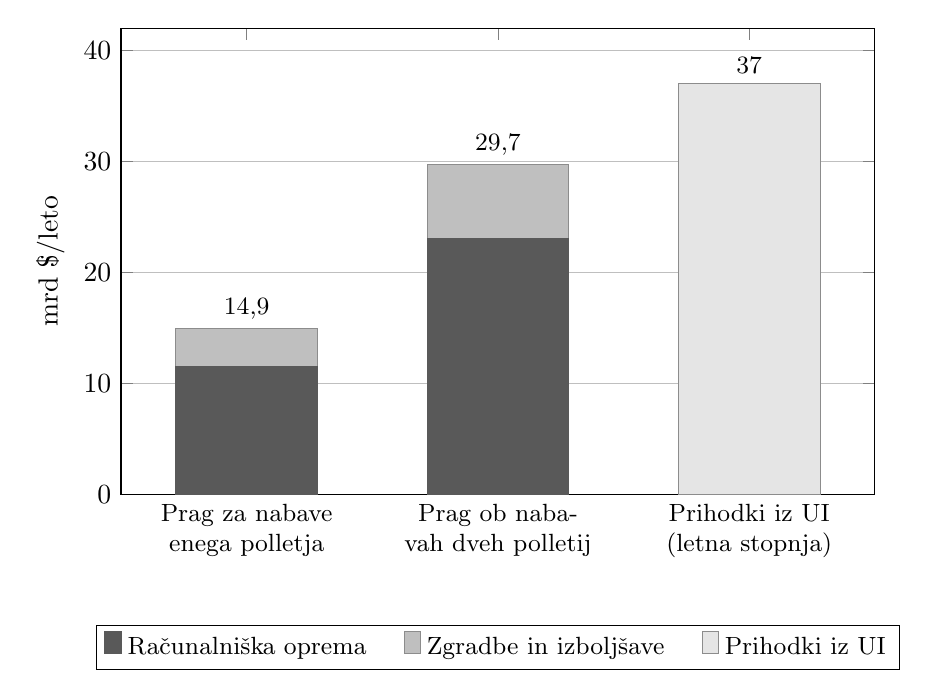
\begin{tikzpicture}
\begin{axis}[
    ybar stacked,
    bar width=1.8cm,
    width=0.92\textwidth,
    height=7.5cm,
    ymin=0, ymax=42,
    ylabel={mrd~\$/leto},
    symbolic x coords={enega,dveh,prihodki},
    xtick=data,
    xticklabels={Prag za nabave enega polletja, Prag ob nabavah dveh polletij, Prihodki iz UI (letna stopnja)},
    xticklabel style={align=center, text width=3.2cm, font=\small},
    enlarge x limits=0.25,
    ymajorgrids=true,
    legend style={at={(0.5,-0.28)}, anchor=north, legend columns=-1, font=\small, /tikz/every even column/.append style={column sep=0.4cm}},
]
\addplot+[fill=black!65, draw=black!65] coordinates {(enega,11.5) (dveh,23.0) (prihodki,0)};
\addplot+[fill=black!25, draw=black!45] coordinates {(enega,3.4) (dveh,6.7) (prihodki,0)};
\addplot+[fill=black!10, draw=black!45] coordinates {(enega,0) (dveh,0) (prihodki,37)};
\legend{Računalniška oprema, Zgradbe in izboljšave, Prihodki iz UI}
\node[above] at (axis cs:enega,14.9) {\small 14,9};
\node[above] at (axis cs:dveh,29.7) {\small 29,7};
\node[above] at (axis cs:prihodki,37) {\small 37};
\end{axis}
\end{tikzpicture}
\caption{Zahtevani donos na nabave in prihodki Microsofta iz UI. Viri: Tabela~\ref{tab:nabave}, lastni izračun; prihodki iz UI: Microsoft, rezultati za FY2026 Q3 (29. 4. 2026), letna stopnja prihodkov 37 mrd~\$.}
\label{fig:zahtevani_donos}
\end{figure}

\subsubsection{Interpretacija}

Računalniška oprema je 59~\% obravnavanih nabav (38,8 od 65,3 mrd~\$), a prispeva 77~\% zahtevanega donosa (11,5 od 14,9 mrd~\$), ker je njen najemni strošek ($R \approx 29{,}7$~\%) več kot dvakrat višji kot pri zgradbah ($R \approx 12{,}7$~\%). Samo nabave iz enega polletja morajo torej vsako leto ustvariti okoli 14,9 mrd~\$ donosa. Ker Microsoft takšne nabave ponavlja, se prag kopiči: ob enakih nabavah v naslednjem polletju bi prag znašal okoli 30 mrd~\$ na leto.

Za oceno velikosti: Microsoft je marca 2026 poročal, da so njegovi prihodki iz UI dosegli letno stopnjo 37 mrd~\$, kar je 123~\% več kot leto prej. Prag za nabave iz dveh polletij (30 mrd~\$) je torej okoli 80~\% teh prihodkov. Primerjava je groba, ker je zahtevani donos kapitala po odštetih drugih stroških (energija, zaposleni), prihodki pa so bruto, poleg tega nabave niso v celoti namenjene UI. Kaže pa red velikosti: prihodki iz UI morajo hitro rasti, da bi pokrili prag, ki ga ustvarjajo ravno nabave opreme.

Model napove, da podjetje investira, dokler je mejni produkt kapitala nad najemnim stroškom, in da je pri opremi z visokim $R$ zahtevani donos bistveno višji kot pri stavbah. To je skladno s podatki: oprema je v nabavah Microsofta 59~\%, a prispeva 77~\% zahtevanega donosa, podjetje pa kljub temu nabavlja opremo v velikem obsegu, kar kaže, da pričakuje hitro rast prihodkov iz UI.

\subsubsection{Občutljivost}

\begin{table}[htbp]
\centering
\caption{Občutljivost zahtevanega donosa na parametre (lastni izračun po modelu, osnova: Tabela~\ref{tab:nabave}).}
\label{tab:obcutljivost}
\small
\begin{tabular}{L{6.2cm}R{1.7cm}R{2.9cm}R{2.0cm}}
\toprule
\textbf{Scenarij (ostali parametri kot v izhodišču)} & \textbf{$R$ opreme} & \textbf{Zahtevani donos (mrd~\$/leto)} & \textbf{Sprememba} \\
\midrule
Izhodišče ($r = 8$~\%, $\delta = 16{,}7$~\%, $\pi_K = -5$~\%) & 29,7~\% & 14,9 & -- \\
$r = 2$~\% (brez premije za tveganje) & 23,7~\% & 10,9 & $-26$~\% \\
$\pi_K = +4{,}2$~\% (cene opreme v 2025) & 20,5~\% & 11,3 & $-24$~\% \\
Življenjska doba 3 leta ($\delta = 33{,}3$~\%) & 46,3~\% & 21,3 & $+44$~\% \\
\bottomrule
\end{tabular}
\end{table}

Prag je najbolj občutljiv na življenjsko dobo opreme: če oprema zdrži tri leta namesto šest, se zviša za 44~\%. Zniža ga odprava premije za tveganje ($-26$~\%) ali rast cen opreme ($-24$~\%). Ob združenih spremembah teh parametrov se prag giblje med 7,4 in 22,6 mrd~\$, torej se razlikuje za več kot trikrat. Odgovor na raziskovalno vprašanje je zato močno odvisen od predpostavk o $\delta$, $\pi_K$ in premiji za tveganje, ki jih ne opazimo neposredno.

\subsubsection{Primeri iz prakse: koliko časa služi oprema za UI?}

Vrednost $\delta$ za opremo UI ni neposredno opazljiva, zato jo podjetja ocenjujejo z računovodsko življenjsko dobo. Primeri kažejo, da je ta ocena sporna in se skozi čas spreminja:

\begin{itemize}
\item Microsoft je z julijem 2022 življenjsko dobo strežnikov in omrežne opreme podaljšal s štirih na šest let, kar je po lastni oceni povečalo operativni dobiček v poslovnem letu 2023 za 3,7 mrd~\$ (Microsoft, 10-K za FY2022). Podobno sta Alphabet (leta 2023) in Oracle (2025) življenjsko dobo podaljšala na šest let, Meta pa večino strežnikov od januarja 2025 odpisuje 5,5 leta.
\item Amazon je leta 2022 življenjsko dobo strežnikov podaljšal s štirih na pet let, leta 2025 pa je za del opreme skrajšal s šest na pet let in kot razlog navedel hiter razvoj UI.
\item Vlagatelj Michael Burry trdi, da je produktni cikel čipov UI le dve do tri leta, podjetja pa jih odpisujejo pet do šest let. Nasprotna stran navaja, da GPU lahko donosno deluje okoli šest let, saj starejšo opremo uporabijo za manj zahtevne naloge.
\end{itemize}

Tabela~\ref{tab:zivljenjska_doba} prikazuje, kaj te ocene pomenijo za zahtevani donos na nabave Microsofta iz Tabele~\ref{tab:nabave} ($r = 8$~\%, $\pi_K = -5$~\%; zgradbe nespremenjene).

\begin{table}[htbp]
\centering
\caption{Zahtevani donos na nabave iz Tabele~\ref{tab:nabave} glede na življenjsko dobo opreme (lastni izračun po modelu; življenjske dobe iz 10-K poročil podjetij in javnih izjav).}
\label{tab:zivljenjska_doba}
\small
\begin{tabular}{L{4.2cm}R{1.4cm}R{1.6cm}R{2.6cm}R{2.8cm}}
\toprule
\textbf{Življenjska doba opreme} & $\delta$ & \textbf{$R$ opreme} & \textbf{Zahtevani donos (mrd~\$/leto)} & \textbf{Sprememba glede na 6 let} \\
\midrule
6 let (Microsoft, Alphabet, Oracle) & 16,7~\% & 29,7~\% & 14,9 & -- \\
5,5 leta (Meta) & 18,2~\% & 31,2~\% & 15,5 & $+0{,}6$ mrd~\$ ($+4$~\%) \\
5 let (Amazon, del opreme) & 20,0~\% & 33,0~\% & 16,1 & $+1{,}3$ mrd~\$ ($+9$~\%) \\
4 leta & 25,0~\% & 38,0~\% & 18,1 & $+3{,}2$ mrd~\$ ($+22$~\%) \\
3 leta (Burry) & 33,3~\% & 46,3~\% & 21,3 & $+6{,}5$ mrd~\$ ($+44$~\%) \\
\bottomrule
\end{tabular}
\end{table}

Tabela pokaže, da se prag donosa z vsakim letom krajše življenjske dobe zviša za okoli 0,6 do 3 mrd~\$, in sicer vse hitreje. Razlika med ocenami podjetij (5 do 6 let) je razmeroma majhna: eno leto krajša doba zviša prag za 1,3 mrd~\$, kar je enako učinku dveh odstotnih točk višje obrestne mere. Razlika med uradnimi ocenami in Burryjevo (3 leta) pa je velika: prag je za 44~\% višji. Prag donosa je torej močno odvisen od ocene življenjske dobe, ki jo podjetja same določajo. Pri tem računovodska odločitev sama ne spremeni ekonomskega praga, spremeni pa poročani dobiček, zato je ključno, katera ocena je resnična.

% --------------------------------------------------
\subsection{Ali so pričakovanja donosov upravičena? Prag rentabilnosti}
% --------------------------------------------------

Model nam omogoča, da raziskovalno vprašanje prevedemo v preprost test: naložba je upravičena, če je donos kapitala (MPK, pomnožen z zalogo) vsaj enak najemnemu strošku. Za nabave opreme in zgradb iz drugega polletja 2025 je prag ob osnovnih predpostavkah okoli 14,9 mrd~\$ na leto (Tabela~\ref{tab:nabave}). Ker Microsoft takšne nabave ponavlja, vzamemo še prag ob enakih nabavah v dveh polletjih (dvakratnik) in ga primerjamo z letno stopnjo prihodkov Microsofta iz UI (37 mrd~\$, marec 2026). Tabela~\ref{tab:test} prikazuje rezultat za tri scenarije (parametri posameznega scenarija so v prvem stolpcu tabele).

\begin{table}[htbp]
\centering
\caption{Test upravičenosti naložb Microsofta v UI (lastni izračun; prihodki iz UI: Microsoft, rezultati za FY2026 Q3, letna stopnja 37 mrd~\$).}
\label{tab:test}
\small
\begin{tabular}{L{5.2cm}R{2.7cm}R{2.7cm}R{3.0cm}}
\toprule
\textbf{Scenarij} & \textbf{Prag za nabave enega polletja (mrd~\$)} & \textbf{Prag ob dveh polletjih (mrd~\$)} & \textbf{Prag kot delež prihodkov iz UI (37 mrd~\$)} \\
\midrule
Optimistični ($r = 2$~\%, $\pi_K = +4{,}2$~\%) & 7,4 & 14,8 & 40~\% \\
Osnovni ($r = 8$~\%, $\delta = 16{,}7$~\%, $\pi_K = -5$~\%) & 14,9 & 29,7 & 80~\% \\
Pesimistični ($r = 10$~\%, $\delta = 33{,}3$~\%) & 22,6 & 45,2 & 122~\% \\
\bottomrule
\end{tabular}
\end{table}

Tudi v optimističnem scenariju bi moral kapital ustvariti okoli 40~\% današnjih prihodkov iz UI, v osnovnem 80~\%, v pesimističnem pa več, kot jih Microsoft danes ustvari (122~\%). Pričakovanja donosov so torej upravičena le, če prihodki iz UI še naprej hitro rastejo: v zadnjem letu so se po Microsoftovih navedbah več kot podvojili ($+123$~\%), in če bi se podvojili še enkrat, bi osnovni prag znašal okoli 40~\% prihodkov. Pri slabših predpostavkah o življenjski dobi in premiji za tveganje pa že današnja raven prihodkov ne bi zadoščala.

Pri razlagi testa moramo biti previdni: zahtevani donos je donos kapitala po odštetih drugih stroških poslovanja. Prihodki iz storitev UI morajo biti zato večji od praga, ker iz njih podjetje plačuje tudi električno energijo, zaposlene in druge vložke. Poleg tega nabave niso v celoti namenjene UI, prag pa velja za vsako leto posebej: oprema, ki zastara v petih ali šestih letih, mora donos prinašati takoj, ne šele čez deset let.

% --------------------------------------------------
\subsection{Ireverzibilnost investicij}
% --------------------------------------------------

Osnovni model predpostavlja, da lahko podjetje kapital kadar koli proda. Tu pa velja, da je del investicije pogosto izgubljen (angl. \textit{sunk cost}), zato se podjetje lahko znajde v položaju $F'(K) < r + \delta$: kapitala je preveč, a ga ne more prodati (prosojnica 41). To je pri UI pomembno, ker se specializirani procesorji težko preprodajo po prvotni vrednosti. Primerjava z optičnimi vlakni ob koncu devetdesetih let kaže razliko: tudi tam je bilo naložb preveč, a je kapital z nizko amortizacijo obstal in so ga izkoristili drugi. Pri GPU z visokim $\delta$ napačna ocena povpraševanja pomeni hitro izgubo vrednosti, zato je tveganje preinvestiranja večje.



% ==================================================
% VIRI (vsi viri so v datoteki viri.bib)
% ==================================================
% Viri, ki so navedeni v seznamu, a jih besedilo ne citira z ukazom \cite:
\nocite{StanfordAIIndex2026,OECD2026,FederalReserve2026,
        Microsoft10K2022,Microsoft2026Q3,FREDDFII10,BLSPPI,
        Verdict2025,iTiger2025,CUBEResearch,Grobovsek2026,Polanec2014}

\setbox0\vbox{\bibliographystyle{plainnat}\bibliography{viri}}

\end{document}


